
\documentclass[border=10pt, 12pt]{standalone}
\usepackage[svgnames]{xcolor}
\usepackage{amsmath}
\usepackage{pgfplots}
\pgfplotsset{compat=newest}
\usepackage[sfdefault]{FiraSans}
\usepackage{FiraMono}
\renewcommand*\familydefault{\sfdefault}
\begin{document}
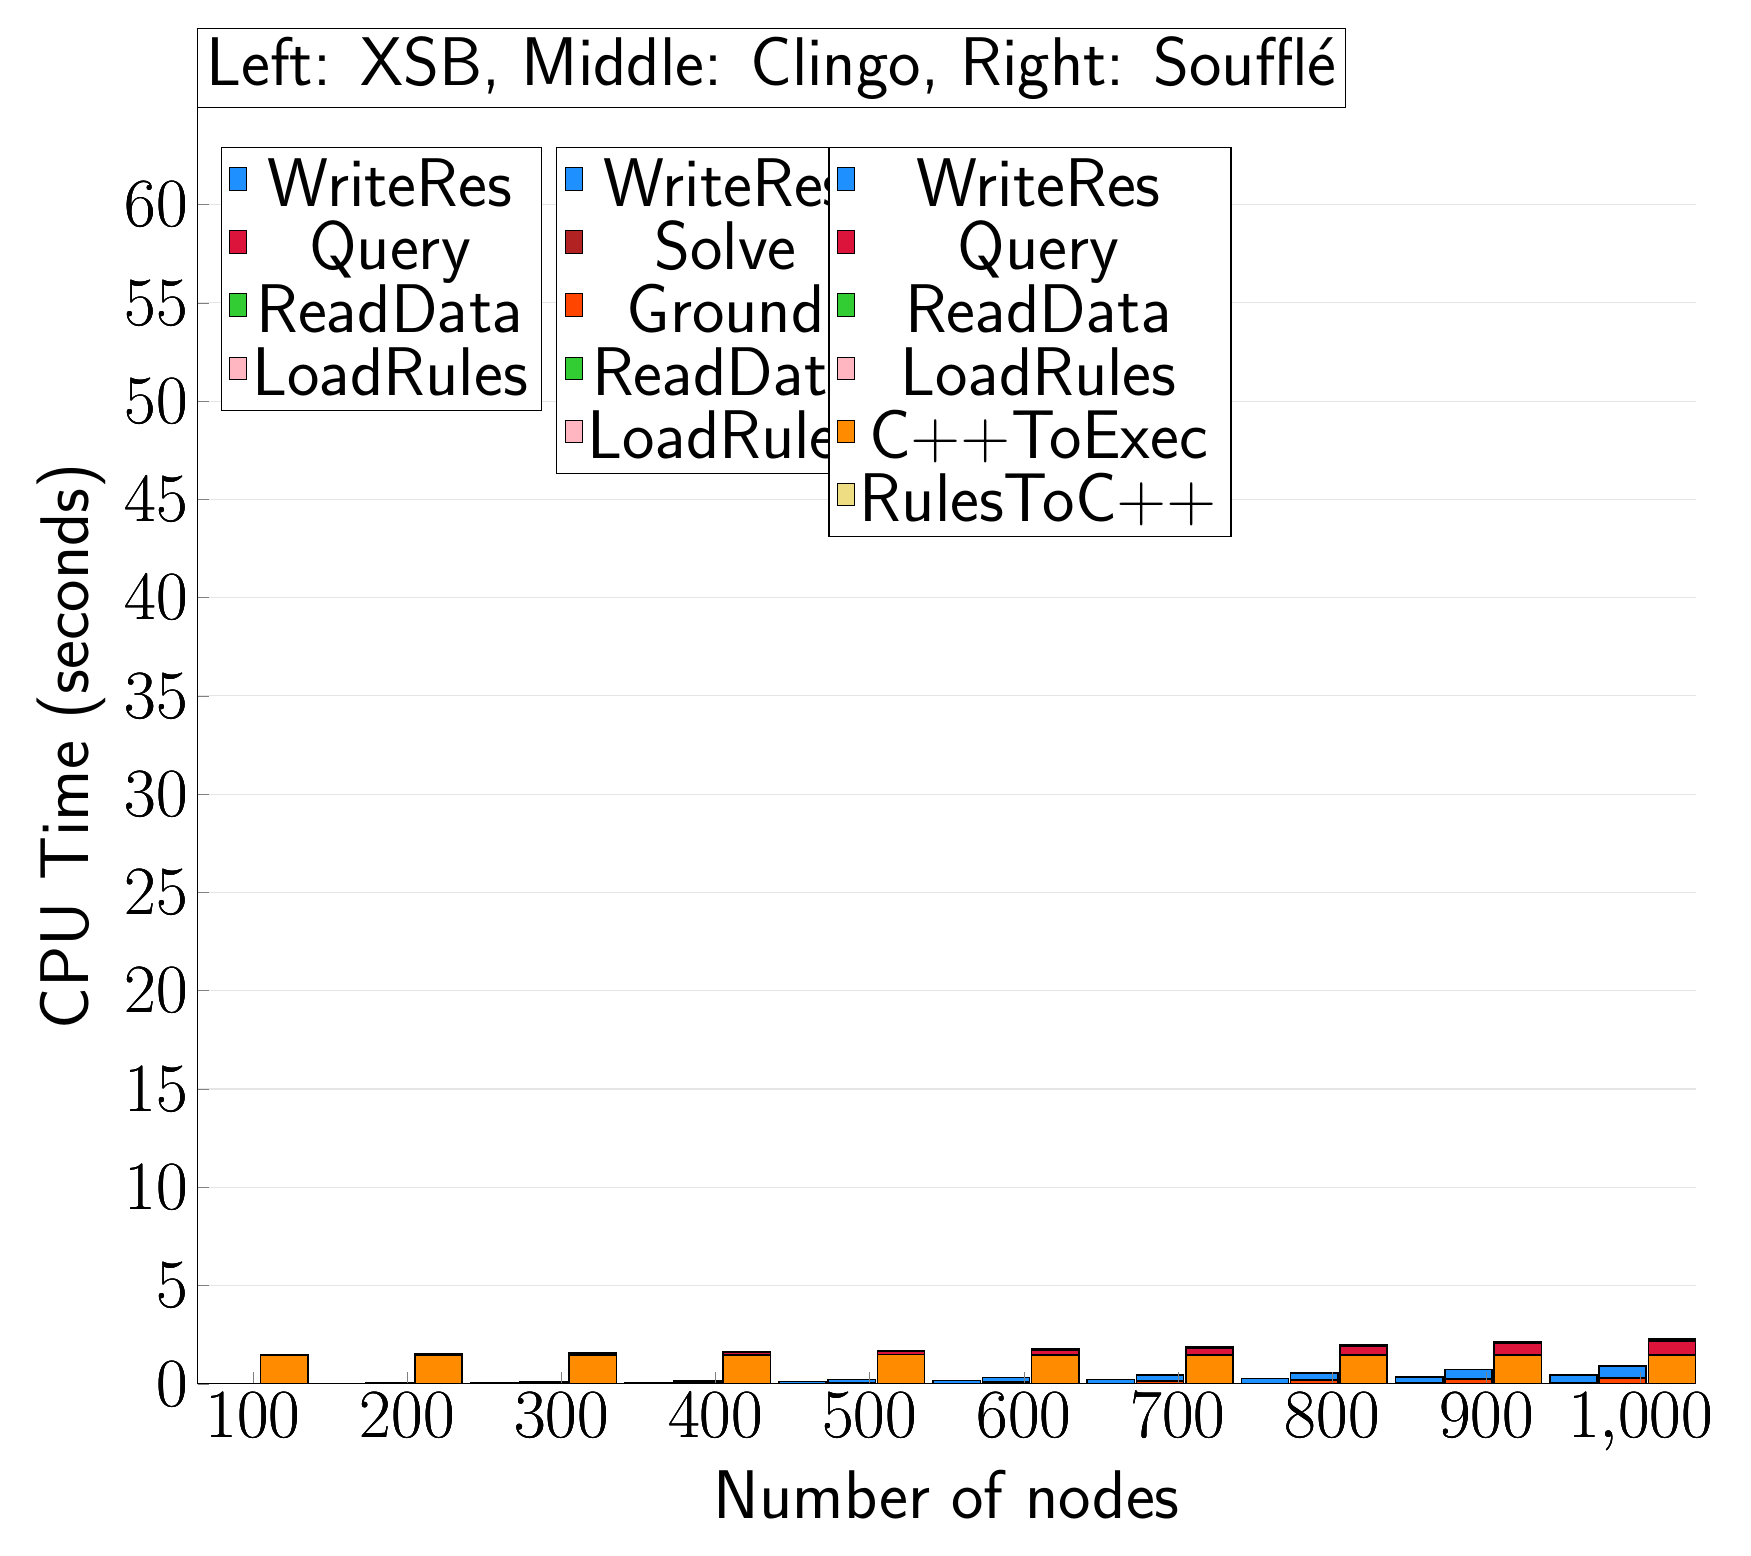
\begin{tikzpicture}
                        \begin{axis}[bar shift=-24.3pt, 
   ybar stacked,
   width=1.7\textwidth,
   bar width=0.6cm,
   ymajorgrids, tick align=inside,
   major grid style={draw=gray!20},
   xtick=data,
   ymin=0, ymax=64.8926,
   axis x line*=bottom,
   axis y line*=left,
   enlarge x limits=0.04,
   legend style={
       at={(0.23, 0.97)},
       anchor=north east,
       legend columns=1,
       font=\Huge,
   },
   ylabel={CPU Time (seconds)},
   xlabel={Number of nodes},
   label style={font=\Huge},
   tick label style={font=\Huge},
]
\addlegendimage{fill=DodgerBlue, draw=black, line width=0.2pt}
\addlegendentry{WriteRes}
\addlegendimage{fill=Crimson, draw=black, line width=0.2pt}
\addlegendentry{Query}
\addlegendimage{fill=LimeGreen, draw=black, line width=0.2pt}
\addlegendentry{ReadData}
\addlegendimage{fill=LightPink, draw=black, line width=0.2pt}
\addlegendentry{LoadRules}
\addplot +[fill=LightPink, draw=black, line width=0.55pt] coordinates {
(100, 0.0005567999999999999)
(200, 0.0005536000000000002)
(300, 0.0005528000000000002)
(400, 0.0005545999999999999)
(500, 0.0005551999999999998)
(600, 0.0005589999999999998)
(700, 0.0005606)
(800, 0.0005548000000000005)
(900, 0.0005612)
(1000, 0.0005553999999999995)
};
\addplot +[fill=LimeGreen, draw=black, line width=0.55pt] coordinates {
(100, 0.0002038000000000002)
(200, 0.00028739999999999983)
(300, 0.0003535999999999998)
(400, 0.0004377999999999992)
(500, 0.0005127999999999999)
(600, 0.0005992000000000003)
(700, 0.0006758000000000001)
(800, 0.0007487999999999998)
(900, 0.0008525999999999997)
(1000, 0.0009120000000000002)
};
\addplot +[fill=Crimson, draw=black, line width=0.55pt] coordinates {
(100, 0.0003948)
(200, 0.0015192)
(300, 0.0033526)
(400, 0.0059786)
(500, 0.0094226)
(600, 0.013517600000000001)
(700, 0.018346599999999998)
(800, 0.023782)
(900, 0.0306152)
(1000, 0.0374298)
};
\addplot +[fill=DodgerBlue, draw=black, line width=0.55pt] coordinates {
(100, 0.004068400000000001)
(200, 0.016179199999999998)
(300, 0.0366398)
(400, 0.0644362)
(500, 0.10132719999999999)
(600, 0.14564880000000002)
(700, 0.1976786)
(800, 0.2565528)
(900, 0.32599199999999995)
(1000, 0.3998938)
};
\end{axis}

\begin{axis}[bar shift=-6.5pt, 
   ybar stacked,
   width=1.7\textwidth,
   bar width=0.6cm,
   ymajorgrids, tick align=inside,
   major grid style={draw=none},
   xtick=data,
   ymin=0, ymax=64.8926,
   axis x line*=none,
   axis y line*=none,
   enlarge x limits=0.04,
   legend style={
       at={(0.454, 0.97)},
       anchor=north east,
       legend columns=1,
       font=\Huge,
   },
   label style={font=\Huge},
   tick label style={font=\Huge},
]
\addlegendimage{fill=DodgerBlue, draw=black, line width=0.2pt}
\addlegendentry{WriteRes}
\addlegendimage{fill=FireBrick, draw=black, line width=0.2pt}
\addlegendentry{Solve}
\addlegendimage{fill=OrangeRed, draw=black, line width=0.2pt}
\addlegendentry{Ground}
\addlegendimage{fill=LimeGreen, draw=black, line width=0.2pt}
\addlegendentry{ReadData}
\addlegendimage{fill=LightPink, draw=black, line width=0.2pt}
\addlegendentry{LoadRules}
\addplot +[fill=LightPink, draw=black, line width=0.55pt] coordinates {
(100, 0.0)
(200, 0.0)
(300, 0.0)
(400, 0.0)
(500, 0.0)
(600, 0.0)
(700, 0.0)
(800, 0.0)
(900, 0.0)
(1000, 0.0)
};
\addplot +[fill=LimeGreen, draw=black, line width=0.55pt] coordinates {
(100, 0.0)
(200, 0.0)
(300, 0.0)
(400, 0.0)
(500, 0.0)
(600, 0.0)
(700, 0.0)
(800, 0.0)
(900, 0.0)
(1000, 0.0)
};
\addplot +[fill=OrangeRed, draw=black, line width=0.55pt] coordinates {
(100, 0.0)
(200, 0.010000000000000009)
(300, 0.020000000000000018)
(400, 0.040000000000000036)
(500, 0.068)
(600, 0.09400000000000003)
(700, 0.14400000000000002)
(800, 0.182)
(900, 0.23199999999999998)
(1000, 0.29800000000000004)
};
\addplot +[fill=FireBrick, draw=black, line width=0.55pt] coordinates {
(100, 0.0)
(200, 0.0)
(300, 0.0)
(400, 0.003999999999999981)
(500, 0.0020000000000000018)
(600, 0.014000000000000009)
(700, 0.016000000000000014)
(800, 0.018000000000000016)
(900, 0.027999999999999987)
(1000, 0.03200000000000001)
};
\addplot +[fill=DodgerBlue, draw=black, line width=0.55pt] coordinates {
(100, 0.010000000000000009)
(200, 0.020000000000000018)
(300, 0.06)
(400, 0.09600000000000002)
(500, 0.15800000000000003)
(600, 0.20999999999999996)
(700, 0.27799999999999997)
(800, 0.36000000000000004)
(900, 0.4620000000000001)
(1000, 0.57)
};
\end{axis}

\begin{axis}[bar shift=11.3pt, 
   ybar stacked,
   width=1.7\textwidth,
   bar width=0.6cm,
   ymajorgrids, tick align=inside,
   major grid style={draw=none},
   xtick=data,
   ymin=0, ymax=64.8926,
   axis x line*=none,
   axis y line*=none,
   enlarge x limits=0.04,
   legend style={
       at={(0.69, 0.97)},
       anchor=north east,
       legend columns=1,
       font=\Huge,
   },
   label style={font=\Huge},
   tick label style={font=\Huge},
]
\addlegendimage{fill=DodgerBlue, draw=black, line width=0.2pt}
\addlegendentry{WriteRes}
\addlegendimage{fill=Crimson, draw=black, line width=0.2pt}
\addlegendentry{Query}
\addlegendimage{fill=LimeGreen, draw=black, line width=0.2pt}
\addlegendentry{ReadData}
\addlegendimage{fill=LightPink, draw=black, line width=0.2pt}
\addlegendentry{LoadRules}
\addlegendimage{fill=DarkOrange, draw=black, line width=0.2pt}
\addlegendentry{C++ToExec}
\addlegendimage{fill=LightGoldenrod, draw=black, line width=0.2pt}
\addlegendentry{RulesToC++}
\addplot +[fill=LightGoldenrod, draw=black, line width=0.55pt] coordinates {
(100, 0.0020000000000000005)
(200, 0.010000000000000002)
(300, 0.006000000000000001)
(400, 0.0020000000000000005)
(500, 0.008000000000000002)
(600, 0.006000000000000001)
(700, 0.008000000000000002)
(800, 0.006000000000000001)
(900, 0.006000000000000001)
(1000, 0.0)
};
\addplot +[fill=DarkOrange, draw=black, line width=0.55pt] coordinates {
(100, 1.468)
(200, 1.464)
(300, 1.466)
(400, 1.466)
(500, 1.472)
(600, 1.464)
(700, 1.464)
(800, 1.462)
(900, 1.464)
(1000, 1.472)
};
\addplot +[fill=LightPink, draw=black, line width=0.55pt] coordinates {
(100, 0.0001516)
(200, 0.0001504)
(300, 0.0001518)
(400, 0.0001672)
(500, 0.000149)
(600, 0.0001544)
(700, 0.000153)
(800, 0.0001474)
(900, 0.00016219999999999999)
(1000, 0.0001602)
};
\addplot +[fill=LimeGreen, draw=black, line width=0.55pt] coordinates {
(100, 0.0009021999999999999)
(200, 0.0012797999999999998)
(300, 0.0017138000000000001)
(400, 0.0018856)
(500, 0.0023184)
(600, 0.0026596000000000002)
(700, 0.0031200000000000004)
(800, 0.0034156)
(900, 0.0038294)
(1000, 0.0043748)
};
\addplot +[fill=Crimson, draw=black, line width=0.55pt] coordinates {
(100, 0.0137654)
(200, 0.042230000000000004)
(300, 0.0782196)
(400, 0.12041539999999999)
(500, 0.18126119999999998)
(600, 0.2559458)
(700, 0.3446002)
(800, 0.44887560000000004)
(900, 0.5677639999999999)
(1000, 0.7062354)
};
\addplot +[fill=DodgerBlue, draw=black, line width=0.55pt] coordinates {
(100, 0.0025544)
(200, 0.0058687999999999995)
(300, 0.0099484)
(400, 0.0172828)
(500, 0.0267668)
(600, 0.038532)
(700, 0.05272980000000001)
(800, 0.0690892)
(900, 0.086214)
(1000, 0.1071094)
};
\end{axis}


\node[anchor=south, draw, fill=white] at (rel axis cs:0.42,1) {\Huge Left: XSB, Middle: Clingo, Right: Soufflé};
\end{tikzpicture}
\end{document}
                    